\documentclass[11pt,a4paper]{article}
\usepackage[utf8]{inputenc}
\usepackage[T1]{fontenc}
\usepackage{amsmath,amsfonts,amssymb}
\usepackage{graphicx}
\usepackage{geometry}
\usepackage{fancyhdr}
\usepackage{setspace}
\usepackage{booktabs}
\usepackage{hyperref}
\usepackage{enumitem}
\usepackage{float}
\usepackage{caption}
\usepackage{subcaption}
\usepackage{array}
\usepackage{tabularx}

% Custom commands
\newcommand{\titlerule}{\noindent\makebox[\linewidth]{\rule{0.7\textwidth}{0.4pt}}}

% Page geometry
\geometry{margin=1in}

% Header/Footer style
\pagestyle{fancy}
\fancyhf{}

% List settings - slightly more spacing
\setlist{itemsep=2pt, parsep=2pt}

% Caption settings
\captionsetup{font=normalsize, labelfont=bf, skip=8pt}

% Hyperlinks
\hypersetup{colorlinks=true, linkcolor=blue, urlcolor=cyan, citecolor=blue}

% Equation spacing
\setlength{\abovedisplayskip}{12pt}
\setlength{\belowdisplayskip}{12pt}
\setlength{\abovedisplayshortskip}{8pt}
\setlength{\belowdisplayshortskip}{8pt}

% Paragraph spacing
\setlength{\parskip}{6pt}

\begin{document}

%=============================================================================
% TITLE PAGE
%=============================================================================
\begin{titlepage}
\newgeometry{margin=1in}
\pagestyle{empty}

% Logos with proper spacing
\begin{minipage}[t]{0.45\textwidth}
    \flushleft
    
\includegraphics[width=4cm]{logo_carthage.png}
\end{minipage}
\hfill
\begin{minipage}[t]{0.45\textwidth}
    \flushright
    
\includegraphics[width=5cm]{logo_supcom.png}
\end{minipage}

\vspace{1.5cm}

\centering
{\LARGE\bfseries Carthage University}\\[0.3cm]
{\Large Higher School of Communication of Tunis}

\vfill


\vspace{1.5cm}

\titlerule\\[0.5cm]
{\LARGE\bfseries Electric Vehicle Routing Optimization}\\[0.3cm]
{\Large Deep Reinforcement Learning for Energy-Minimizing EVRP}\\[0.5cm]
\titlerule

\vfill

\begin{center}
\begin{minipage}{0.65\textwidth}
\raggedright
{\large\bfseries Authors:}\\[0.2cm]
{\Large Salem Fradi}\\
{\Large Dhia Elhak Ezzeddini}\\[1cm]
{\large\bfseries Supervisor:}\\[0.2cm]
{\Large Dr. Ferdaoues Chaabane}\\[1cm]
{\large\bfseries Host Company:}\\[0.2cm]
{\Large Sagemcom}
\end{minipage}
\end{center}

\vfill

{\Large Academic Year: 2025--2026}

\restoregeometry
\end{titlepage}

%=============================================================================
% ACKNOWLEDGMENTS
%=============================================================================
\cleardoublepage
\newgeometry{margin=1in}
\pagestyle{empty}
\vspace*{2cm}

\begin{center}
\section*{Acknowledgments}
\addcontentsline{toc}{section}{Acknowledgments}
\end{center}

\vspace{1cm}

\begin{large}
\begin{onehalfspacing}
We express our deepest gratitude to our supervisor, Dr. Ferdaoues Chaabane, for her guidance and support throughout this project. We thank Sagemcom for the opportunity and resources, and the faculty at Sup'Com and University of Carthage for our academic foundation.
\end{onehalfspacing}
\end{large}

\vfill
\restoregeometry

%=============================================================================
% TABLE OF CONTENTS
%=============================================================================
\cleardoublepage
\pagenumbering{roman}
\fancyhf{}
\lhead{Contents}
\rhead{\thepage}
\tableofcontents

%=============================================================================
% MAIN CONTENT
%=============================================================================
\cleardoublepage
\pagenumbering{arabic}
\setcounter{page}{1}
\fancyhf{}
\lhead{EV Routing Optimization}
\rhead{\thepage}
\onehalfspacing

%-----------------------------------------------------------------------------
\section{Introduction}
%-----------------------------------------------------------------------------

\subsection{Context and Motivation}

The rapid adoption of Electric Vehicles (EVs) presents challenges for logistics systems. Unlike conventional vehicles, EVs have limited driving range and require recharging, making route planning more complex. The \textbf{Electric Vehicle Routing Problem (EVRP)} extends classical VRP by incorporating battery capacity, charging station locations, and energy consumption patterns.

\subsection{Problem Statement}

We address the \textbf{Energy-Minimizing EVRP (EM-EVRP)}, minimizing total energy consumption while satisfying:
\begin{itemize}
    \item Customer demand fulfillment
    \item Vehicle capacity constraints
    \item Battery State of Charge (SOC) limitations
    \item Time window requirements
    \item Real-world road network constraints
\end{itemize}

Specifically, we consider a scenario where a fleet of EVs must serve $n$ customers from a central depot, potentially visiting charging stations to maintain sufficient battery levels.

\subsection{Objectives}

The main objectives are:
\begin{enumerate}
    \item Formulate a comprehensive Mixed Integer Linear Programming (MILP) model for EM-EVRP
    \item Implement and evaluate classical optimization baselines including Google OR-Tools, Hill Climbing, Simulated Annealing, and Ant Colony Optimization
    \item Develop a Deep Reinforcement Learning (DRL) solution using attention-based neural networks
    \item Design a scalable real-world deployment pipeline integrating:
    \begin{itemize}
        \item \textbf{K-means clustering} for customer grouping
        \item \textbf{Dijkstra's algorithm} for shortest path computation on road networks
        \item \textbf{OSRM} for production-grade street-level routing
    \end{itemize}
    \item Create an interactive dashboard for visualization and real-world deployment
\end{enumerate}

%-----------------------------------------------------------------------------
\section{Mathematical Formulation}
%-----------------------------------------------------------------------------

\subsection{Sets and Indices}

Table~\ref{tab:sets} defines the sets used in our formulation.

\begin{table}[H]
\centering
\caption{Sets and indices notation}
\label{tab:sets}
\begin{tabular}{@{}cl@{}}
\toprule
\textbf{Symbol} & \textbf{Description} \\
\midrule
$N$ & Set of all nodes $\{0, 1, \ldots, n\}$ where $0$ is the depot \\
$C$ & Set of customers $C = N \setminus \{0\}$ \\
$S$ & Set of charging stations \\
$K$ & Set of vehicles $\{1, \ldots, m\}$ \\
$R$ & Set of trip indices $\{1, \ldots, R_{\max}\}$ \\
\bottomrule
\end{tabular}
\end{table}

\subsection{Network Parameters}

Table~\ref{tab:network_params} presents the network-related parameters.

\begin{table}[H]
\centering
\caption{Network parameters}
\label{tab:network_params}
\begin{tabular}{@{}cl@{}}
\toprule
\textbf{Symbol} & \textbf{Description} \\
\midrule
$d_i$ & Demand of customer $i$ \\
$Q_k$ & Capacity of vehicle $k$ \\
$t_{ij}$ & Travel time on arc $(i, j)$ \\
$[a_i, b_i]$ & Time window at node $i$ \\
$g_i$ & Service time at node $i$ \\
$T_{\max}$ & Time horizon \\
$M$ & Big-M constant for linearization \\
\bottomrule
\end{tabular}
\end{table}

\subsection{EV Energy Parameters}

Table~\ref{tab:energy_params} lists the parameters for the physics-based energy model.

\begin{table}[H]
\centering
\caption{EV energy parameters}
\label{tab:energy_params}
\begin{tabular}{@{}cl@{}}
\toprule
\textbf{Symbol} & \textbf{Description} \\
\midrule
$m_c$ & Curb mass of the vehicle (kg) \\
$C_d$ & Aerodynamic drag coefficient \\
$C_r$ & Rolling resistance coefficient \\
$\rho$ & Air density (kg/m$^3$) \\
$A$ & Frontal area of the vehicle (m$^2$) \\
$g$ & Gravitational acceleration (m/s$^2$) \\
$\alpha_{ij}$ & Slope angle on arc $(i, j)$ \\
$v_{ij}$ & Average speed on arc $(i, j)$ (m/s) \\
$\varphi_d$ & Motor efficiency for propulsion \\
$\varphi_r$ & Motor efficiency for regeneration \\
$\phi_d$ & Battery discharge efficiency \\
$\phi_r$ & Battery charge efficiency (regenerative braking) \\
\bottomrule
\end{tabular}
\end{table}

\subsection{Decision Variables}

Table~\ref{tab:variables} describes the decision variables in our model.

\begin{table}[H]
\centering
\caption{Decision variables}
\label{tab:variables}
\begin{tabular}{@{}cl@{}}
\toprule
\textbf{Variable} & \textbf{Description} \\
\midrule
$x_{ijk}^r \in \{0,1\}$ & 1 if vehicle $k$ traverses arc $(i,j)$ in trip $r$ \\
$y_{ik}^r \in \{0,1\}$ & 1 if customer $i$ is served by vehicle $k$ in trip $r$ \\
$z_k \in \{0,1\}$ & 1 if vehicle $k$ is used \\
$\tau_{ik}^r \geq 0$ & Service start time at node $i$ by vehicle $k$ in trip $r$ \\
$w_{ik}^r \geq 0$ & MTZ subtour elimination variable \\
\bottomrule
\end{tabular}
\end{table}

\subsection{Energy Consumption Model}

The physics-based energy model considers vehicle mass, aerodynamic drag, rolling resistance, and gravitational effects.

\textbf{Total mass on arc $(i,j)$:}
\begin{equation}
m_{ij} = m_c + u_{ij}
\end{equation}
where $u_{ij}$ is the cargo load.

\textbf{Power required for traversal:}
\begin{equation}
P_{ij} = \left( m_{ij} a + m_{ij} g \left( \sin\alpha_{ij} + C_r \cos\alpha_{ij} \right) + \frac{1}{2} C_d \rho A v_{ij}^2 \right) v_{ij}
\end{equation}

\textbf{Energy consumption:}
\begin{equation}
E_{ij} =
\begin{cases}
\phi_d \varphi_d P_{ij} t_{ij} & \text{if } P_{ij} \geq 0 \text{ (propulsion)} \\
\phi_r \varphi_r P_{ij} t_{ij} & \text{if } P_{ij} < 0 \text{ (regenerative braking)}
\end{cases}
\end{equation}

\subsection{MILP Formulation}

\textbf{Objective Function:} Minimize total energy consumption
\begin{equation}
\min \sum_{k \in K} \sum_{r \in R} \sum_{(i,j)} E_{ij} \cdot x_{ijk}^r
\end{equation}

\textbf{Subject to:}

\textit{Each customer served exactly once:}
\begin{equation}
\sum_{k \in K} \sum_{r \in R} y_{ik}^r = 1, \quad \forall i \in C
\end{equation}

\textit{Flow conservation:}
\begin{equation}
\sum_{j} x_{ijk}^r = y_{ik}^r = \sum_{j} x_{jik}^r, \quad \forall i \in C, k \in K, r \in R
\end{equation}

\textit{Vehicle capacity:}
\begin{equation}
\sum_{i \in C} d_i \cdot y_{ik}^r \leq Q_k, \quad \forall k \in K, r \in R
\end{equation}

\textit{Subtour elimination (MTZ):}
\begin{equation}
w_{ik}^r - w_{jk}^r + |C| \cdot x_{ijk}^r \leq |C| - 1, \quad \forall i,j \in C, k \in K, r \in R
\end{equation}

\textit{Time window constraints:}
\begin{equation}
a_i \cdot y_{ik}^r \leq \tau_{ik}^r \leq b_i + M(1 - y_{ik}^r), \quad \forall i \in C, k \in K, r \in R
\end{equation}

%-----------------------------------------------------------------------------
\section{Baseline Optimization Methods}
%-----------------------------------------------------------------------------

\subsection{Google OR-Tools}

Google OR-Tools is an open-source optimization suite providing powerful constraint programming and routing solvers. Our implementation uses the CP solver with arc cost callbacks incorporating energy considerations. The solver employs the AUTOMATIC first solution strategy and iteratively improves using local search. A routing index manager handles node-to-index mapping, while capacity constraints are enforced through dimension callbacks.

\subsection{Hill Climbing}

Hill Climbing is a local search algorithm that iteratively improves solutions by making incremental changes. Starting from an initial solution generated by nearest neighbor heuristic, it explores the neighborhood using:
\begin{itemize}
    \item \textbf{2-opt:} Reverse a segment of the route
    \item \textbf{Or-opt:} Relocate a sequence of customers
    \item \textbf{Exchange:} Swap customers between routes
\end{itemize}

The algorithm terminates when no improving neighbor exists:
\begin{equation}
S' \gets \arg\min_{s \in \mathcal{N}(S)} f(s); \quad \text{if } f(S') < f(S) \text{ then } S \gets S', \text{ else terminate}
\end{equation}

\subsection{Simulated Annealing}

Simulated Annealing (SA) extends Hill Climbing by accepting uphill moves to escape local optima. The acceptance probability is controlled by temperature:
\begin{equation}
P(\text{accept}) =
\begin{cases}
1 & \text{if } \Delta E < 0 \\
\exp\left( -\Delta E / T \right) & \text{otherwise}
\end{cases}
\end{equation}

The temperature follows geometric cooling:
\begin{equation}
T_{k+1} = \alpha \cdot T_k, \quad \alpha \in [0.9, 0.99]
\end{equation}

This allows exploration at high temperatures and exploitation at low temperatures, enabling escape from local minima that trap Hill Climbing.

\subsection{Ant Colony Optimization}

ACO is inspired by ant foraging behavior, using pheromone trails to guide search. The transition probability from node $i$ to $j$ is:
\begin{equation}
p_{ij}^a = \frac{[\tau_{ij}]^\alpha [\eta_{ij}]^\beta}{\sum_{l \in \mathcal{N}_i} [\tau_{il}]^\alpha [\eta_{il}]^\beta}
\end{equation}
where $\tau_{ij}$ is the pheromone level and $\eta_{ij} = 1/c_{ij}$ is the heuristic information (inverse of cost).

Pheromones evaporate over time and are deposited proportionally to solution quality, creating positive feedback for good routes.

%-----------------------------------------------------------------------------
\section{Deep Reinforcement Learning Approach}
%-----------------------------------------------------------------------------

\subsection{MDP Formulation}

We formulate routing as a Markov Decision Process (MDP) with the components shown in Table~\ref{tab:mdp}.

\begin{table}[H]
\centering
\caption{MDP components for EVRP}
\label{tab:mdp}
\begin{tabular}{@{}lp{10cm}@{}}
\toprule
\textbf{Component} & \textbf{Description} \\
\midrule
State $s_t$ & Partial solution, current vehicle position, remaining capacity, and SOC \\
Action $a_t$ & Next node to visit (customer, charging station, or depot) \\
Reward $r_t$ & Negative energy consumption for the traversed arc \\
Policy $\pi_\theta$ & Neural network parameterized by weights $\theta$ \\
\bottomrule
\end{tabular}
\end{table}

\subsection{Architecture}

\textbf{Encoder:} Multi-head self-attention processes the input graph:
\begin{equation}
h_i^{(l)} = \text{BN}\left( h_i^{(l-1)} + \text{MHA}\left( h_i^{(l-1)}, H^{(l-1)} \right) \right)
\end{equation}

This produces node embeddings $H = \{h_1, \ldots, h_n\}$ and graph embedding:
\begin{equation}
\bar{h} = \frac{1}{n} \sum_{i=1}^{n} h_i
\end{equation}

\textbf{Decoder:} Generates routes autoregressively with context:
\begin{equation}
c_t = W_c \left[ \bar{h}; h_{\pi_{t-1}}; \text{cap}_t; \text{SOC}_t \right]
\end{equation}

\textbf{Selection:} Uses attention mechanism:
\begin{equation}
u_{tj} = C \cdot \tanh\left( \frac{q_t \cdot k_j}{\sqrt{d_k}} \right), \quad j \in \mathcal{A}_t \text{ (feasible actions)}
\end{equation}
\begin{equation}
p_\theta(a_t = j | s_t) = \text{softmax}(u_t)_j
\end{equation}

\subsection{Training Algorithm}

We use REINFORCE with rollout baseline for variance reduction. The objective is:
\begin{equation}
J(\theta) = \mathbb{E}_{\pi_\theta}\left[ L(\pi) \right]
\end{equation}
where $L(\pi)$ is the route cost.

The gradient is estimated as:
\begin{equation}
\nabla_\theta J = \mathbb{E}\left[ \left( L(\pi) - b(s) \right) \nabla_\theta \log p_\theta(\pi | s) \right]
\end{equation}
where $b(s)$ is the baseline from a periodically updated policy copy. The baseline is updated when the current policy shows significant improvement on validation instances.

\subsection{EV-Specific Features}

\textbf{SOC Tracking:}
\begin{equation}
\text{SOC}_{t+1} = \text{SOC}_t - \frac{E_{ij}}{E_{\text{battery}}}
\end{equation}

Charging stations are included as optional nodes; the model learns when to visit them.

\textbf{Action Masking:} Ensures feasibility by restricting available actions:
\begin{equation}
\mathcal{A}_t = \left\{ j : d_j \leq \text{cap}_t \land E_{ij} \leq \text{SOC}_t \cdot E_{\text{battery}} \right\}
\end{equation}

%-----------------------------------------------------------------------------
\section{Real-World Deployment Pipeline}
%-----------------------------------------------------------------------------

A critical challenge in deploying DRL-based routing solutions is bridging the gap between models trained on synthetic Euclidean distances and real-world road networks. This section presents our complete pipeline for real-world deployment, integrating K-means clustering, Dijkstra's algorithm, and OSRM (Open Source Routing Machine) to enable practical EV routing on actual street networks.

\subsection{Pipeline Overview}

Our real-world deployment pipeline consists of four main stages:
\begin{enumerate}
    \item \textbf{Customer Grouping:} Partition large customer sets into manageable groups of 10 using K-means clustering
    \item \textbf{Charging Station Assignment:} Assign the 4 nearest charging stations to each customer group
    \item \textbf{Distance Matrix Construction:} Compute real road network distances between all Points of Interest (POIs) using Dijkstra's algorithm or OSRM Table API
    \item \textbf{DRL Inference and Route Projection:} Run the trained model and project optimal routes onto real street geometries
\end{enumerate}

This modular architecture enables scalability: while the DRL model is trained on 10-customer instances, the pipeline can handle arbitrarily large customer sets by intelligent partitioning.

\subsection{K-Means Customer Clustering}

To scale beyond the training configuration of 10 customers, we employ K-means clustering to partition large customer sets into balanced groups.

\textbf{Algorithm:} Given $N$ customer locations $\{c_1, c_2, \ldots, c_N\}$ where $c_i = (\text{lat}_i, \text{lon}_i)$, we compute $k = \lfloor N/10 \rfloor$ clusters:
\begin{equation}
\mu_j = \arg\min_{\mu} \sum_{c_i \in C_j} \|c_i - \mu\|^2, \quad j \in \{1, \ldots, k\}
\end{equation}

\textbf{Balancing:} Standard K-means may produce uneven clusters. We apply a post-processing step to ensure exactly 10 customers per group:
\begin{enumerate}
    \item Assign up to 10 customers to each cluster based on initial K-means labels
    \item Redistribute excess customers to under-filled clusters based on proximity to cluster centroids
    \item Verify each group contains exactly 10 customers
\end{enumerate}

\textbf{Station Assignment:} For each customer group with centroid $\mu_j$, we assign the 4 nearest charging stations from the global station pool:
\begin{equation}
S_j = \arg\min_{S \subset \mathcal{S}, |S|=4} \sum_{s \in S} \|\mu_j - s\|
\end{equation}
where $\mathcal{S}$ is the set of all available charging stations.

\subsection{Road Network Graph Construction}

We construct the underlying road network using OpenStreetMap (OSM) data, processed via OSMnx. The network is represented as a directed multigraph $G = (V, E)$ where:
\begin{itemize}
    \item $V$ is the set of road intersections and endpoints (nodes)
    \item $E$ is the set of road segments (edges) with attributes: length (m), speed limit (km/h), travel time (s), and slope (degrees)
\end{itemize}

\textbf{Edge Attributes:} For each edge $(u, v) \in E$, we store:
\begin{equation}
e_{uv} = \left( L_{uv}, \; v_{uv}, \; T_{uv} = \frac{L_{uv}}{v_{uv}}, \; \theta_{uv} \right)
\end{equation}
where $L_{uv}$ is the length in meters, $v_{uv}$ is the speed in m/s, $T_{uv}$ is the travel time, and $\theta_{uv}$ is the slope angle.

\textbf{Spatial Indexing:} To efficiently locate the nearest graph node for any coordinate, we construct a KD-tree over all node positions:
\begin{equation}
n^* = \arg\min_{n \in V} \left\| (\text{lat}_n, \text{lon}_n) - (\text{lat}_q, \text{lon}_q) \right\|
\end{equation}
This reduces node lookup complexity from $O(|V|)$ to $O(\log |V|)$.

\subsection{Dijkstra's Algorithm for Shortest Paths}

Given the road network graph $G$ and a set of POIs (depot, depot charging, 4 stations, 10 customers = 16 nodes), we construct the complete pairwise distance matrix using Dijkstra's shortest path algorithm.

\textbf{Single-Source Shortest Path:} For source node $s$, Dijkstra's algorithm computes:
\begin{equation}
d(s, v) = \min_{\text{path } P: s \rightsquigarrow v} \sum_{(u,w) \in P} L_{uw}, \quad \forall v \in V
\end{equation}

\textbf{Path Metrics:} For each POI pair $(i, j)$, we compute three metrics along the shortest path:
\begin{align}
D_{ij} &= \sum_{(u,v) \in P_{ij}} L_{uv} \quad \text{(total distance in meters)} \\
T_{ij} &= \sum_{(u,v) \in P_{ij}} T_{uv} \quad \text{(total travel time in seconds)} \\
S_{ij} &= \frac{\sum_{(u,v) \in P_{ij}} \tan(\theta_{uv}) \cdot L_{uv}}{D_{ij}} \quad \text{(length-weighted average slope)}
\end{align}

\textbf{Matrix Construction:} The complete distance matrix $\mathbf{D} \in \mathbb{R}^{16 \times 16}$ requires 240 Dijkstra computations (excluding diagonal). We store the actual paths for later visualization:
\begin{equation}
\text{Paths}_{ij} = [n_1, n_2, \ldots, n_k] \text{ where } n_1 = \text{POI}_i, \; n_k = \text{POI}_j
\end{equation}

\textbf{Implementation:} We use NetworkX's optimized Dijkstra implementation with edge weight set to road segment length:
\begin{verbatim}
    path = nx.shortest_path(G, poi[i], poi[j], weight='length')
\end{verbatim}

\subsection{OSRM Integration for Production Routing}

For production deployment, we integrate the Open Source Routing Machine (OSRM) to obtain real-world routing with consideration for turn restrictions, one-way streets, and traffic patterns.

\textbf{Table API:} Instead of $N^2$ individual routing requests, OSRM's Table API computes the full distance matrix in a single HTTP request:
\begin{verbatim}
    GET /table/v1/driving/{coords}?annotations=distance
\end{verbatim}
where \texttt{coords} is a semicolon-separated list of \texttt{lon,lat} pairs.

\textbf{Route API:} For visualization, we fetch actual street geometries using the Route API:
\begin{verbatim}
    GET /route/v1/driving/{origin};{destination}?geometries=polyline
\end{verbatim}
The response includes an encoded polyline representing the exact street-level path.

\subsection{Coordinate Normalization and Model Input}

The DRL model expects inputs normalized to a $[0, 100]$ coordinate space. We apply affine transformation to POI coordinates:
\begin{align}
x_i &= \frac{\text{lon}_i - \text{lon}_{\min}}{\text{lon}_{\max} - \text{lon}_{\min}} \times 100 \\
y_i &= \frac{\text{lat}_i - \text{lat}_{\min}}{\text{lat}_{\max} - \text{lat}_{\min}} \times 100
\end{align}

Similarly, distances are scaled to match the training distribution:
\begin{equation}
D'_{ij} = \frac{D_{ij}}{D_{\max}} \times 141
\end{equation}
where 141 approximates the maximum Euclidean distance in a $[0,100]^2$ space ($\sqrt{2} \times 100$).

\subsection{Complete Pipeline Workflow}

Algorithm~\ref{alg:pipeline} summarizes the complete real-world routing pipeline.

\begin{table}[H]
\centering
\caption{Real-World EV Routing Pipeline}
\label{alg:pipeline}
\begin{tabular}{@{}p{0.70\textwidth}@{}}
\toprule
\textbf{Algorithm: Real Streets EV Routing Pipeline} \\
\midrule
\textbf{Input:} Customer coordinates $\mathcal{C}$, Station pool $\mathcal{S}$, Depot location $d$, Trained model $\pi_\theta$ \\
\textbf{Output:} Optimized routes with real street geometries \\
\midrule
1. \textbf{Group customers:} $\mathcal{G} \gets \text{KMeans}(\mathcal{C}, k=|\mathcal{C}|/10)$ \\
2. \textbf{Balance groups:} Ensure $|G_i| = 10$ for all $G_i \in \mathcal{G}$ \\
3. \textbf{For each} group $G_i \in \mathcal{G}$: \\
\quad 3.1. Compute centroid $\mu_i = \text{mean}(G_i)$ \\
\quad 3.2. Assign stations $S_i \gets \text{nearest}_4(\mu_i, \mathcal{S})$ \\
\quad 3.3. Build POI list: $P_i = [d, d_{\text{chg}}, S_i, G_i]$ \\
\quad 3.4. Compute distance matrix $\mathbf{D}_i$ via OSRM or Dijkstra \\
\quad 3.5. Normalize coordinates and distances \\
\quad 3.6. Run DRL inference: $\pi_i \gets \pi_\theta(P_i, \mathbf{D}_i)$ \\
\quad 3.7. Fetch street geometries for route segments \\
4. \textbf{Return} all group routes with visualization data \\
\bottomrule
\end{tabular}
\end{table}

%-----------------------------------------------------------------------------
\section{Results and Discussion}
%-----------------------------------------------------------------------------

\subsection{Experimental Setup}

Training data was generated synthetically based on CVRPLIB benchmarks including P-n19-k2, P-n21-k2, P-n40-k5, and P-n51-k10. All experiments were conducted on a workstation equipped with an \textbf{NVIDIA T1000 8GB} GPU and an \textbf{Intel Core i5-12500 3.0 GHz} CPU. The configuration parameters are shown in Table~\ref{tab:config}.

\begin{table}[H]
\centering
\caption{Training configuration}
\label{tab:config}
\begin{tabular}{@{}ll@{}}
\toprule
\textbf{Parameter} & \textbf{Value} \\
\midrule
Number of customers & 10 \\
Number of charging stations & 4 \\
Embedding dimension & 128 \\
Encoder layers & 3 \\
Attention heads & 8 \\
Batch size & 1024 \\
Learning rate & $10^{-4}$ \\
Baseline type & Rollout \\
Initial SOC & 80\% \\
GPU & NVIDIA T1000 8GB \\
CPU & Intel Core i5-12500 @ 3.0 GHz \\
\bottomrule
\end{tabular}
\end{table}

Figure~\ref{fig:synthetic} illustrates a sample synthetic training instance. The data generation follows a structured approach: the depot is placed centrally (coordinates 25--75), charging stations are distributed across four quadrants to ensure coverage, and customer locations are randomly sampled across a $100 \times 100$ grid. Each customer has a randomly assigned demand, and elevation values are generated to simulate realistic terrain variations affecting energy consumption.

\begin{figure}[H]
\centering
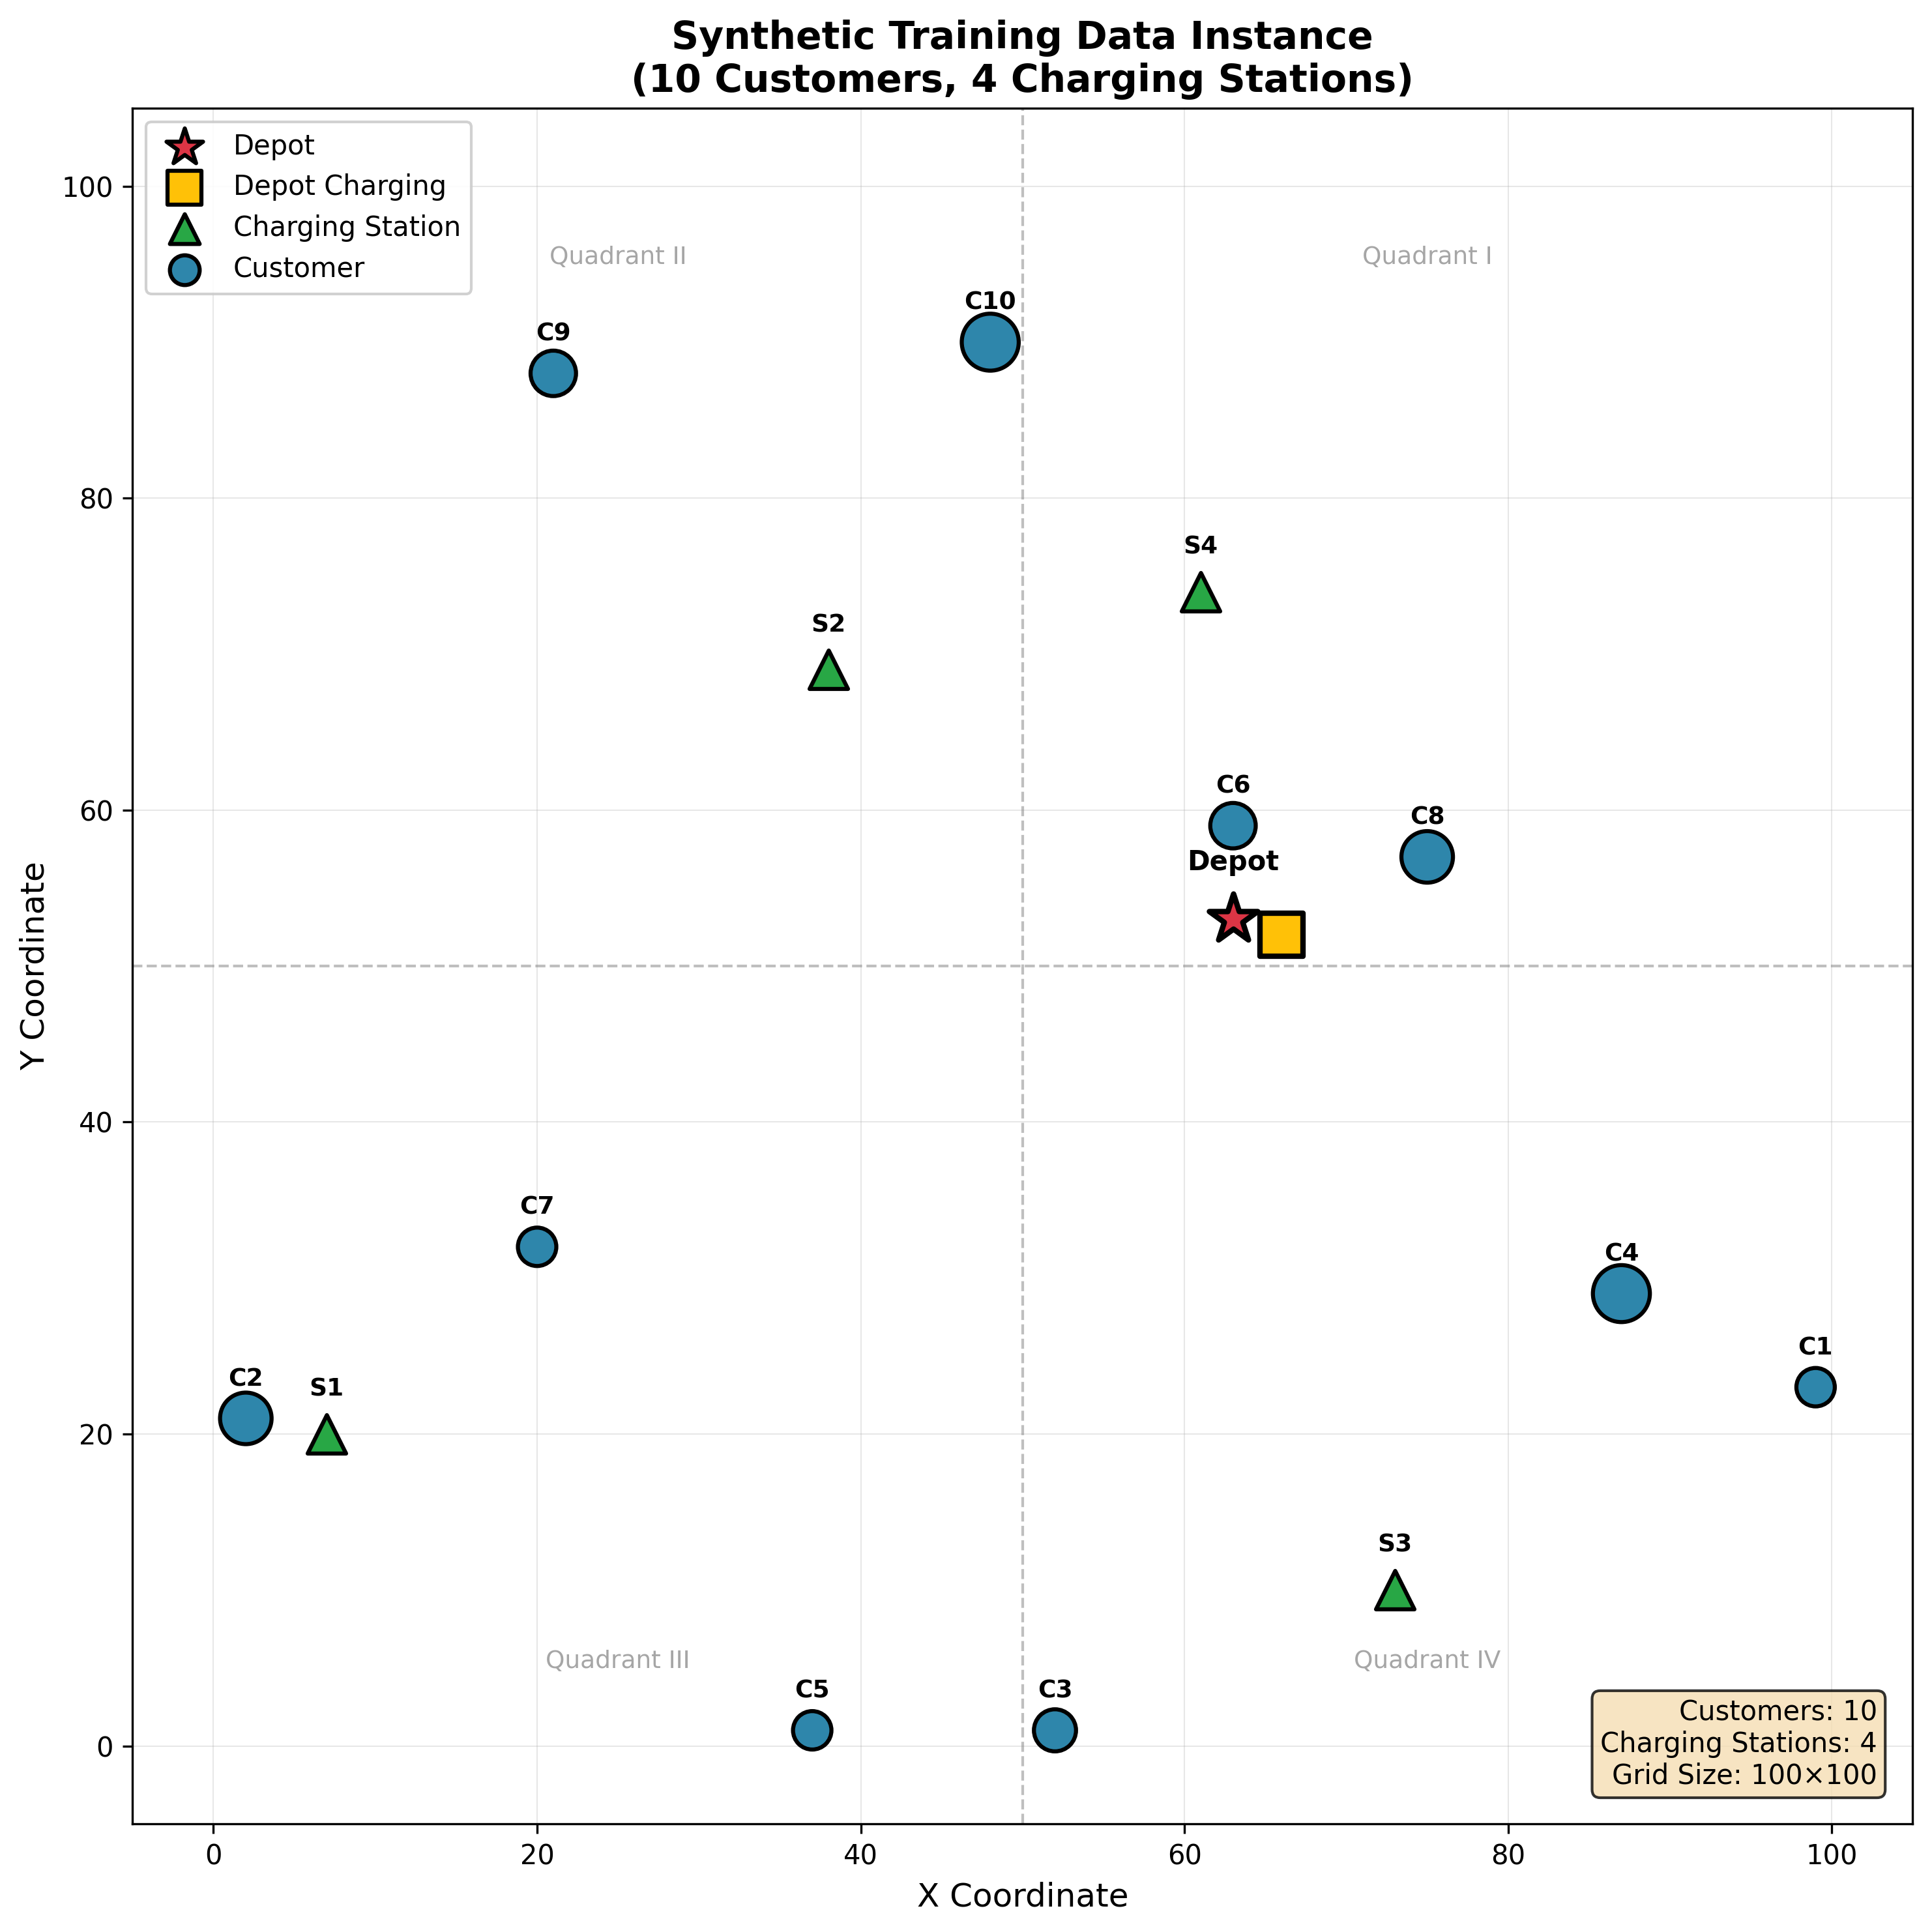
\includegraphics[width=0.40\textwidth]{figures/synthetic_training_data.png}
\caption{Sample synthetic training data instance showing depot, charging stations distributed across quadrants, and customer locations with varying demands}
\label{fig:synthetic}
\end{figure}

\subsection{Training Results}

Figure~\ref{fig:train} shows training and validation rewards over 100 epochs. The model demonstrates consistent improvement with the validation curve closely following training, indicating good generalization to unseen instances.

\begin{figure}[H]
\centering
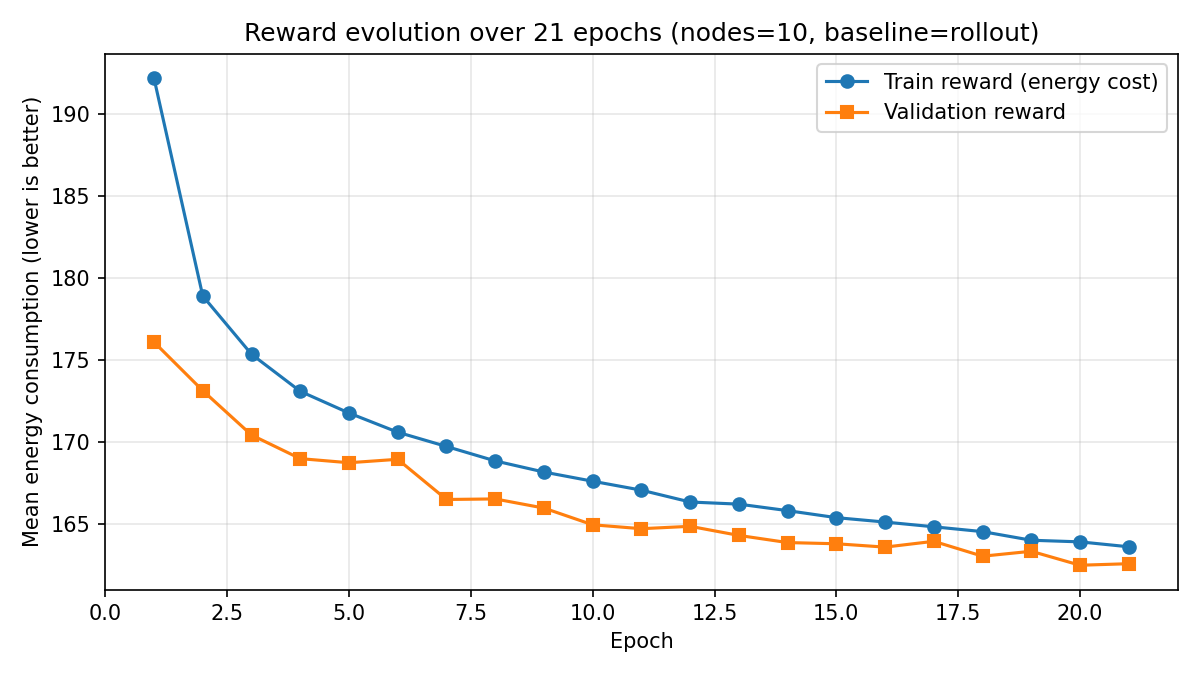
\includegraphics[width=0.6\textwidth]{figures/training_reward.png}
\caption{Training and validation rewards over 100 epochs (10 nodes, rollout baseline)}
\label{fig:train}
\end{figure}

\subsection{Comparison with Baselines}

Table~\ref{tab:comp} compares methods on 10-customer instances. Google OR-Tools achieves the best energy consumption (11.92 kWh) as expected from an exact solver. The DRL approach achieves near-optimal results (12.18 kWh, only 2.2\% gap) with significantly faster inference time (0.5s vs 2.1s), making it suitable for real-time applications where solution speed is critical.

\begin{table}[H]
\centering
\caption{Performance comparison on 10-customer instances}
\label{tab:comp}
\begin{tabular}{@{}lcc@{}}
\toprule
\textbf{Method} & \textbf{Energy (kWh)} & \textbf{Inference Time} \\
\midrule
\textbf{OR-Tools} & \textbf{11.92} & 2.1s \\
DRL & 12.18 & \textbf{0.5s} \\
Ant Colony Optimization & 12.67 & 3.2s \\
Simulated Annealing & 12.89 & 1.5s \\
Hill Climbing & 13.21 & 0.8s \\
\bottomrule
\end{tabular}
\end{table}

\subsection{Dashboard Integration}

We developed an interactive Streamlit dashboard with OpenStreetMap integration that implements the complete real-world deployment pipeline described in Section~5. The dashboard provides:

\begin{itemize}
    \item \textbf{Customer Upload:} CSV file input for customer locations with automatic K-means grouping
    \item \textbf{Interactive Map:} Leaflet-based map showing customers, stations, and depot with clustering visualization
    \item \textbf{Real-Time Optimization:} One-click route optimization using the trained DRL model with real road distances
    \item \textbf{Street-Level Routes:} OSRM-powered route rendering showing actual street paths, not straight lines
    \item \textbf{Energy Analytics:} Per-segment energy consumption breakdown considering distance, elevation, and vehicle load
    \item \textbf{SOC Monitoring:} Real-time battery State of Charge tracking with charging station visit recommendations
\end{itemize}

\textbf{Pipeline Integration:} The dashboard seamlessly integrates all pipeline components:
\begin{enumerate}
    \item Customers are automatically clustered into groups of 10 using K-means
    \item Each group is assigned its 4 nearest charging stations
    \item Distance matrices are computed via OSRM Table API (with Dijkstra fallback)
    \item The DRL model performs inference on normalized inputs
    \item Routes are visualized on OpenStreetMap with actual street geometries
\end{enumerate}

\textbf{Scalability:} By leveraging the K-means grouping strategy, the dashboard can handle hundreds of customers while maintaining the computational efficiency of the 10-customer DRL model. Each group is processed independently, enabling parallel optimization for large-scale deployments.

\begin{figure}[H]
\centering
\begin{subfigure}{0.48\textwidth}
    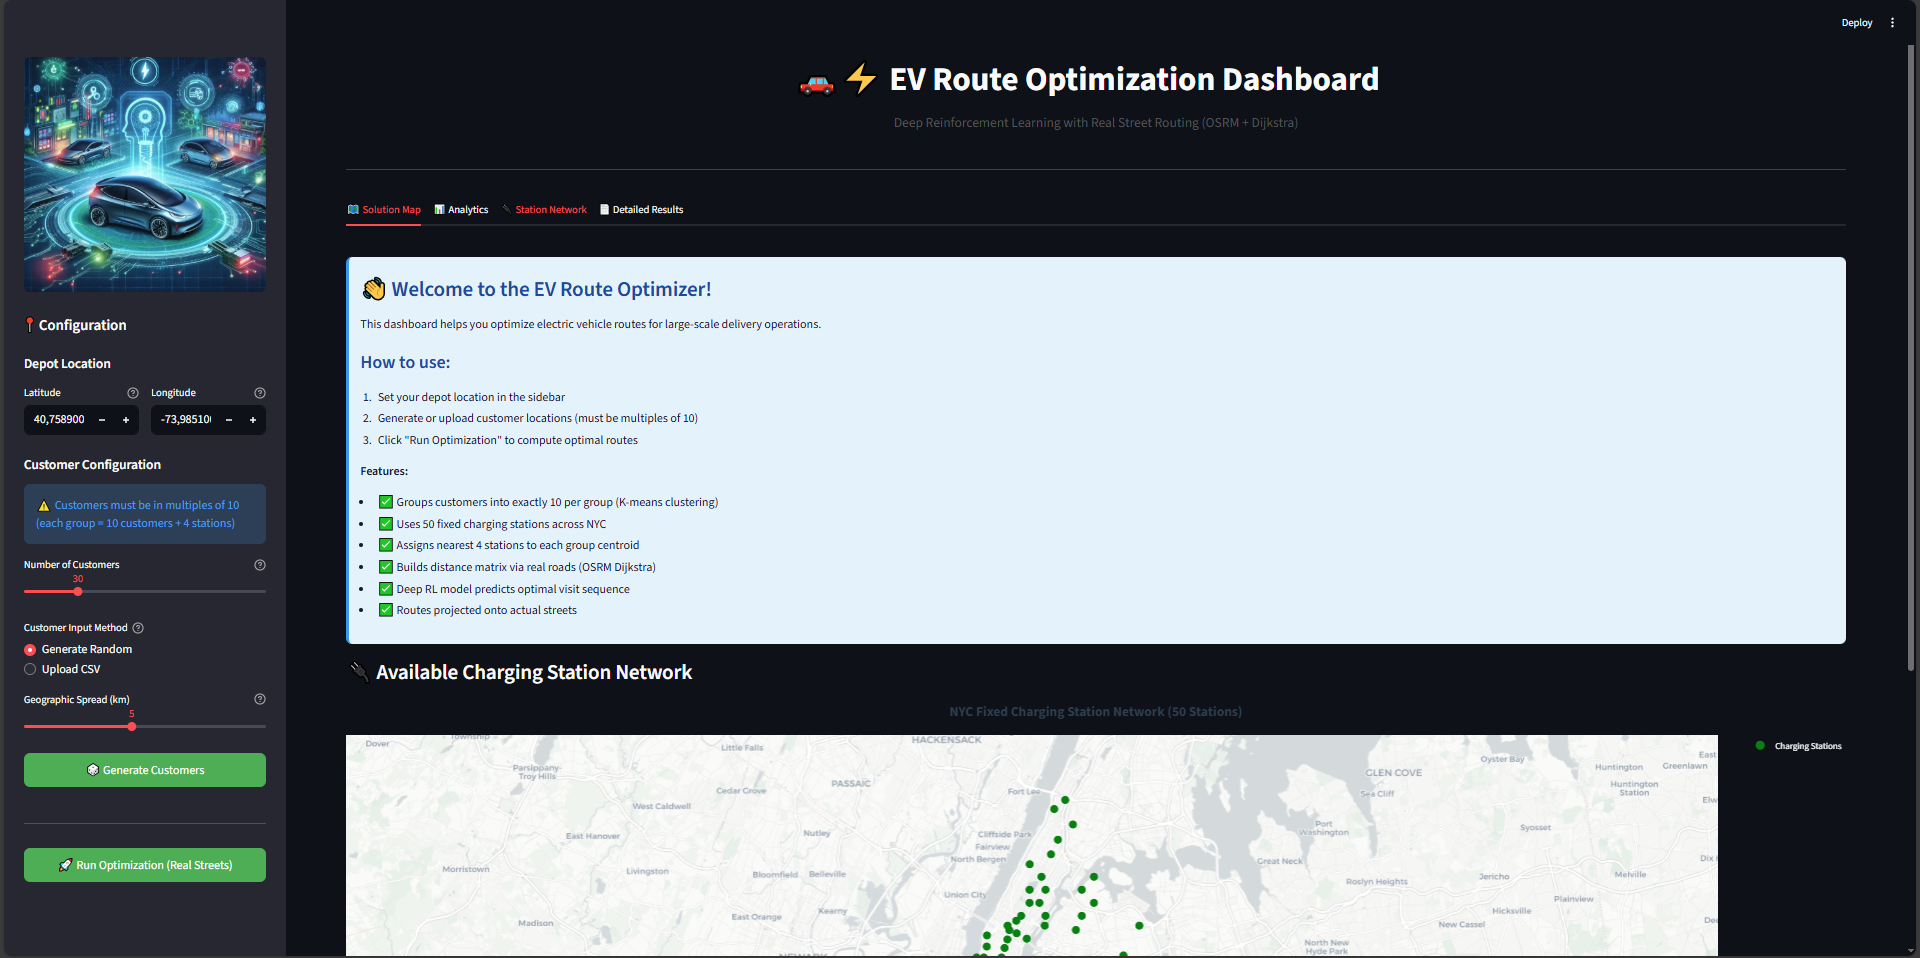
\includegraphics[width=\textwidth]{figures/main_page.PNG}
    \caption{Main interface}
\end{subfigure}
\hfill
\begin{subfigure}{0.48\textwidth}
    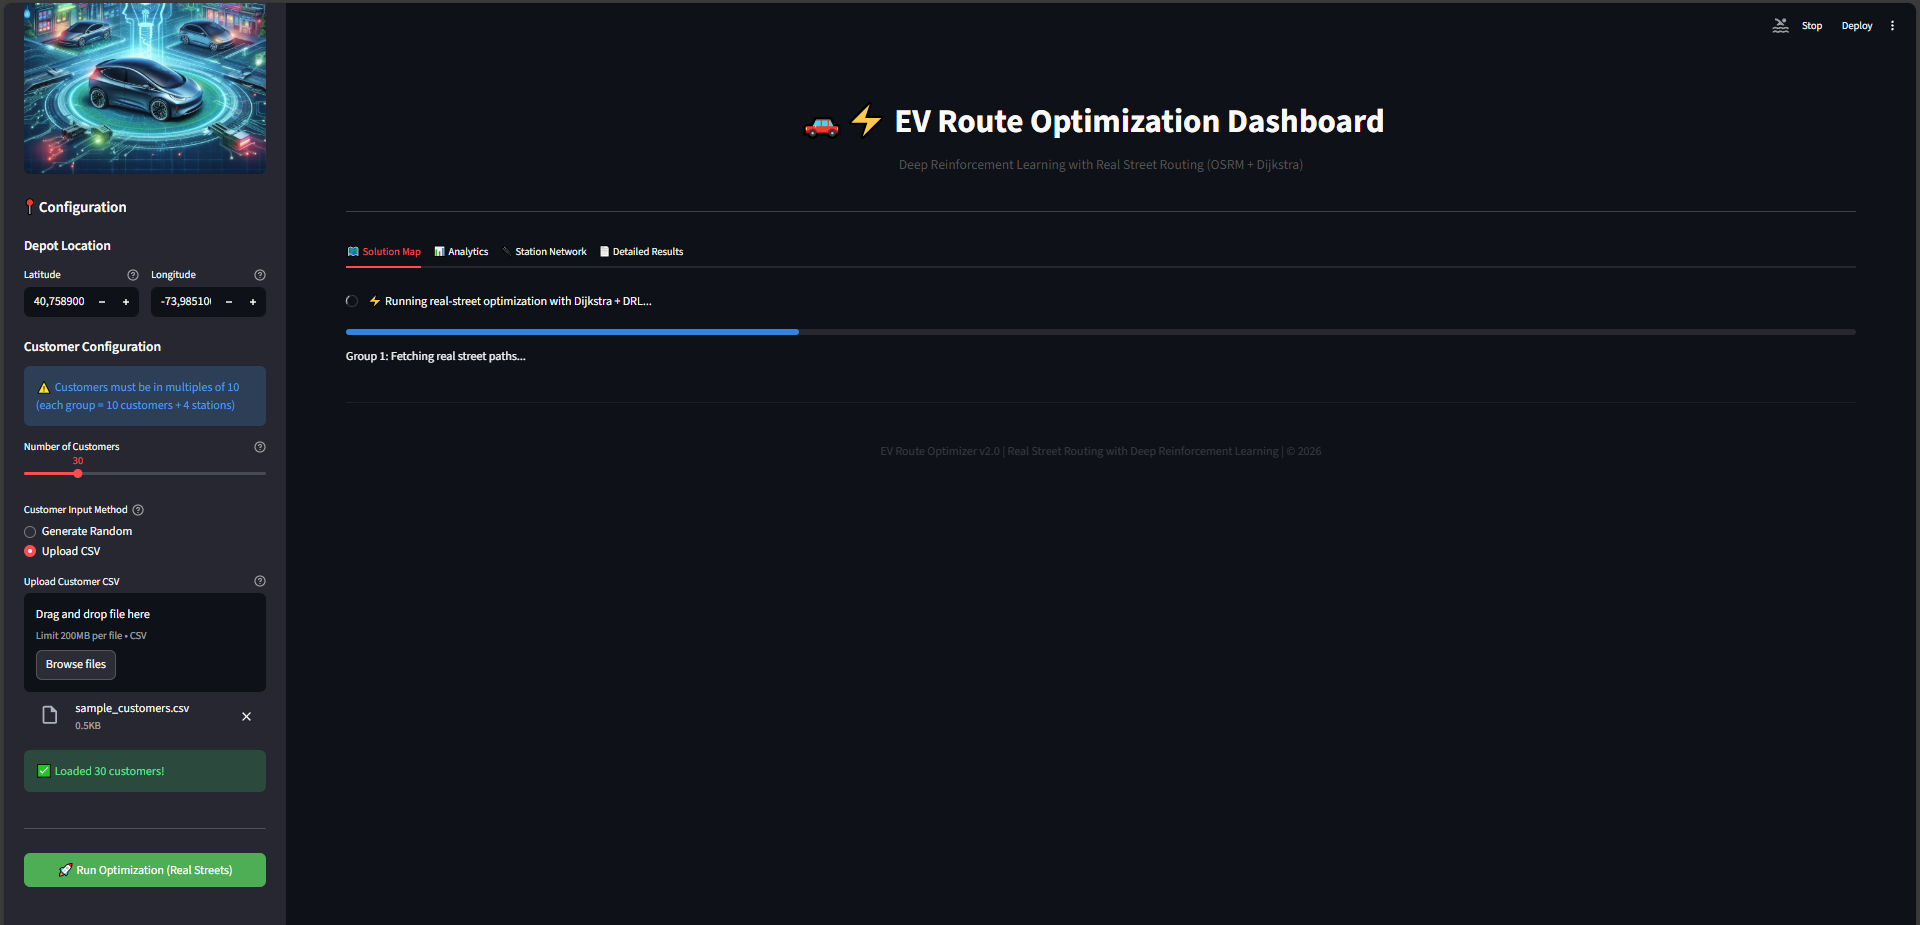
\includegraphics[width=\textwidth]{figures/inference.PNG}
    \caption{Inference view}
\end{subfigure}

\vspace{0.5cm}

\begin{subfigure}{0.48\textwidth}
    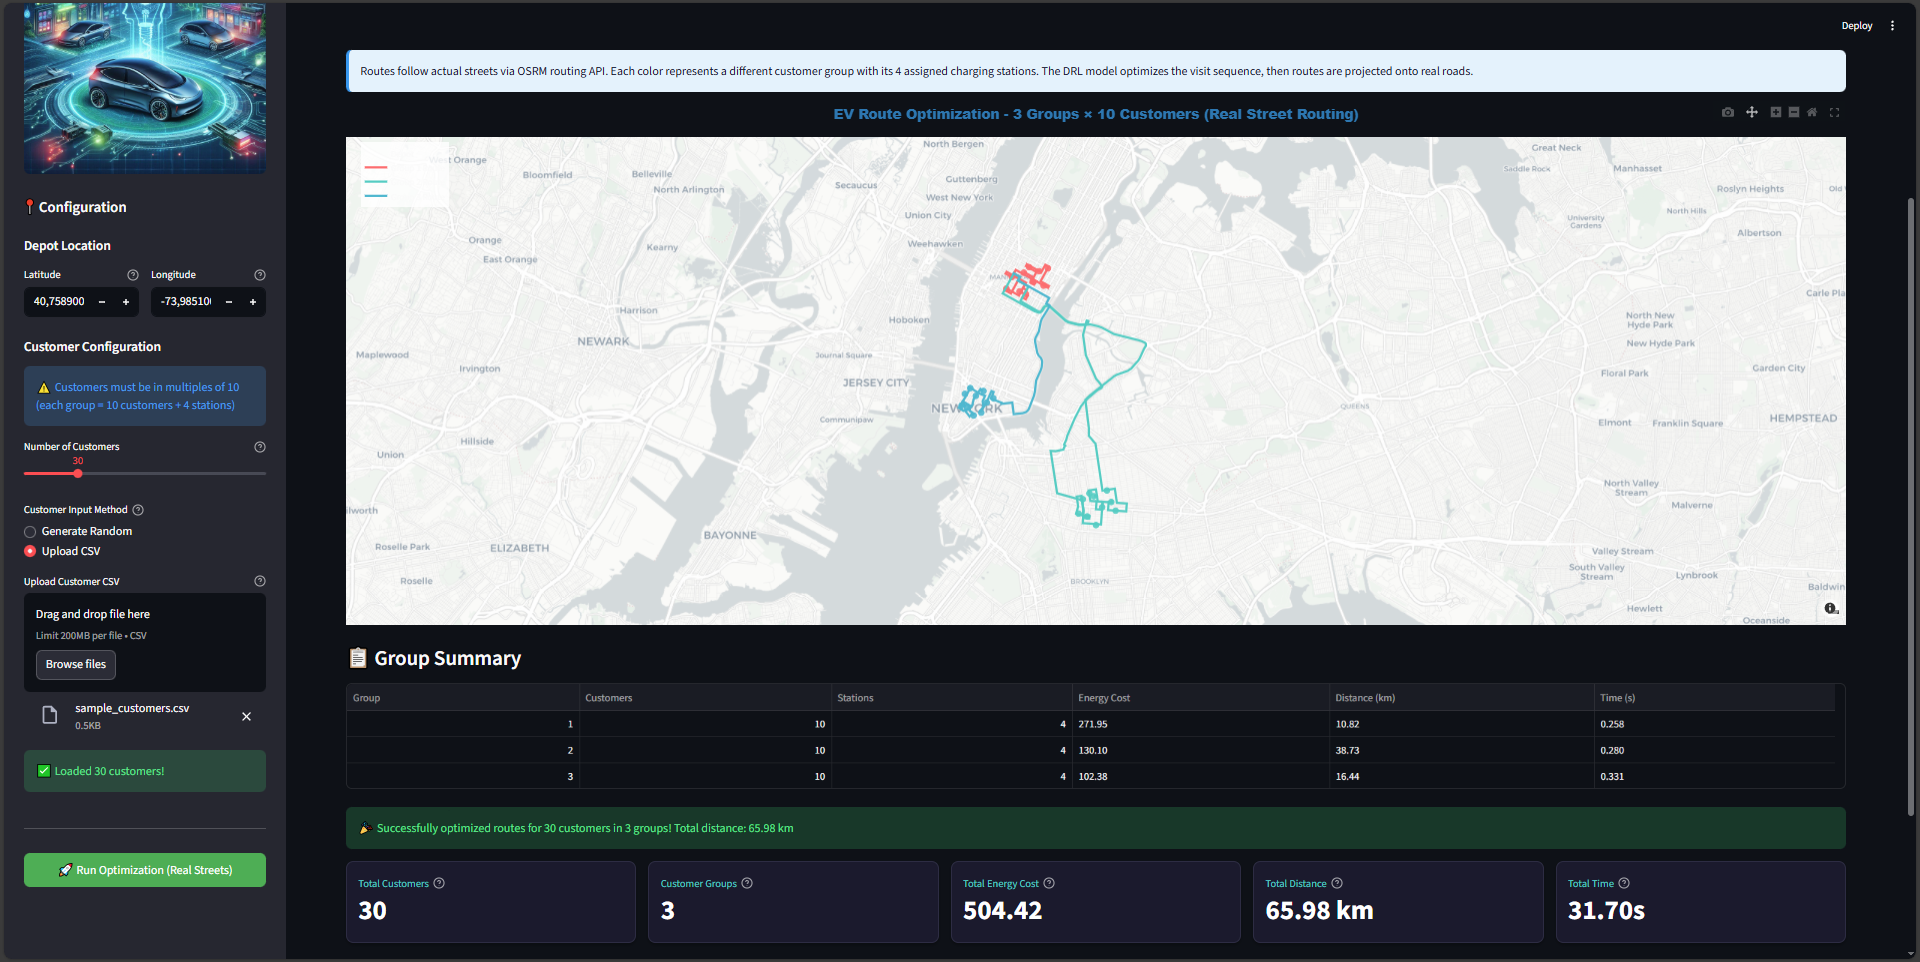
\includegraphics[width=\textwidth]{figures/result.PNG}
    \caption{Optimized routes}
\end{subfigure}
\hfill
\begin{subfigure}{0.48\textwidth}
    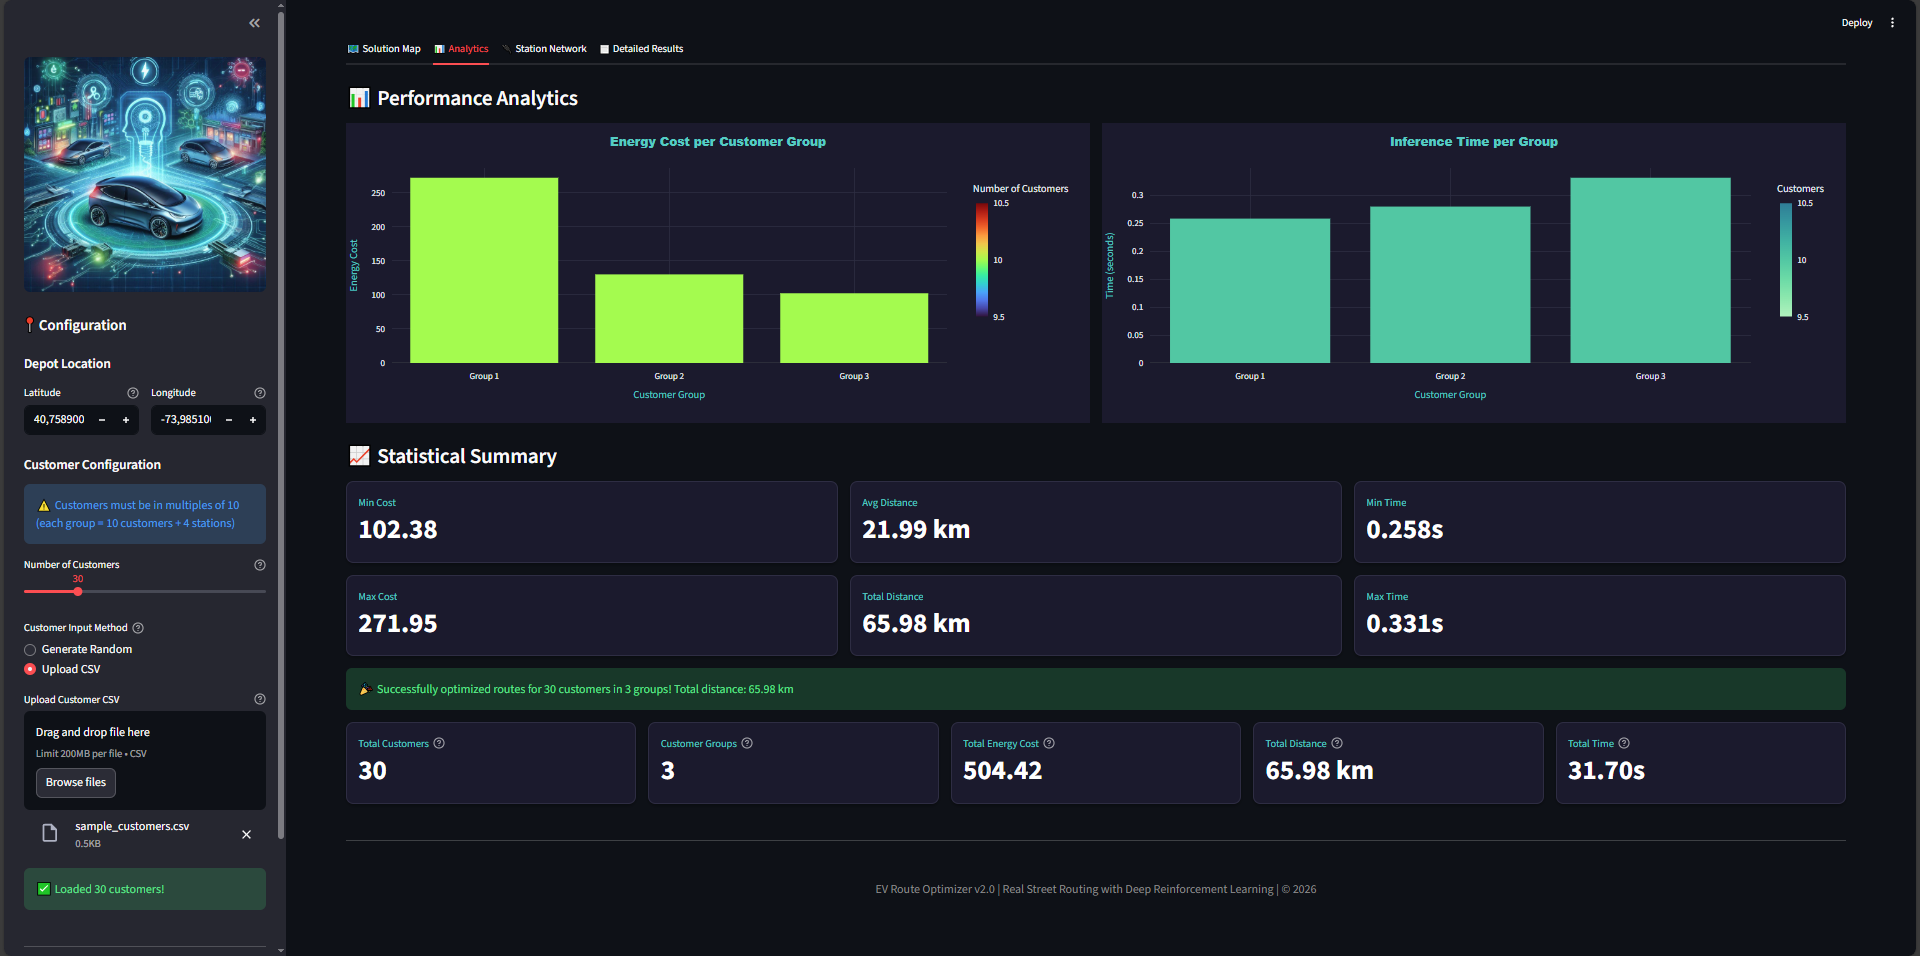
\includegraphics[width=\textwidth]{figures/analytics.PNG}
    \caption{Analytics dashboard}
\end{subfigure}
\caption{Dashboard interfaces for EV route optimization}
\label{fig:dash}
\end{figure}

%-----------------------------------------------------------------------------
\section{Conclusion}
%-----------------------------------------------------------------------------

\subsection{Summary}

This project addressed the Energy-Minimizing Electric Vehicle Routing Problem using Deep Reinforcement Learning, with a complete pipeline for real-world deployment. Our contributions include:
\begin{enumerate}
    \item \textbf{Mathematical Formulation:} Comprehensive MILP formulation incorporating multi-trip capability, time windows, and physics-based energy consumption
    \item \textbf{Baseline Implementations:} Classical optimization methods (OR-Tools, Hill Climbing, Simulated Annealing, ACO) for rigorous benchmarking
    \item \textbf{DRL Model:} Attention-based neural network achieving near-optimal solutions with fast inference
    \item \textbf{Real-World Pipeline:} Novel integration of K-means clustering, Dijkstra's algorithm, and OSRM for scalable deployment on real road networks
    \item \textbf{Interactive Dashboard:} Production-ready visualization tool with street-level routing and energy analytics
\end{enumerate}

\subsection{Key Findings}

\begin{itemize}
    \item The DRL approach generalizes well to unseen instances after training on synthetic data
    \item \textbf{K-means clustering} enables scalability beyond the training configuration by partitioning large customer sets into balanced groups
    \item \textbf{Dijkstra's algorithm} on OSM road networks provides accurate real-world distances while preserving path information for visualization
    \item \textbf{OSRM integration} offers production-grade routing with sub-second response times for complete distance matrices
    \item The attention mechanism effectively captures customer-to-customer relationships
    \item Physics-based energy modeling provides realistic consumption estimates considering aerodynamics, rolling resistance, and regenerative braking
    \item Inference time is significantly lower than iterative optimization methods, making real-time routing feasible
\end{itemize}

\subsection{Future Work}

Several directions could extend this work:
\begin{itemize}
    \item \textbf{Larger Instances:} Training on 50+ customer instances to reduce reliance on clustering
    \item \textbf{Dynamic Scenarios:} Real-time traffic integration and demand updates using live OSRM profiles
    \item \textbf{Multi-Depot Optimization:} Extending the pipeline to support multiple depot locations
    \item \textbf{Heterogeneous Fleets:} Supporting mixed EV types with different battery capacities and consumption profiles
    \item \textbf{Charging Schedule Optimization:} Joint optimization of routing and charging timing based on electricity prices
    \item \textbf{Elevation-Aware Routing:} Integrating digital elevation models (DEM) for more accurate energy predictions on hilly terrain
\end{itemize}

%-----------------------------------------------------------------------------
% REFERENCES
%-----------------------------------------------------------------------------
\newpage
\addcontentsline{toc}{section}{References}
\begin{thebibliography}{99}

% Deep Reinforcement Learning for Routing
\bibitem{kool} W. Kool, H. van Hoof, and M. Welling, ``Attention, Learn to Solve Routing Problems!'' in \emph{Proceedings of the International Conference on Learning Representations (ICLR)}, 2019.

\bibitem{camp} C. Hua, F. Berto, J. Son, S. Kang, C. Kwon, and J. Park, ``CAMP: Collaborative Attention Model with Profiles for Vehicle Routing Problems,'' in \emph{Proceedings of the 24th International Conference on Autonomous Agents and Multiagent Systems (AAMAS)}, Detroit, Michigan, USA, 2025.

\bibitem{tang2023} M. Tang, W. Zhuang, B. Li, H. Liu, Z. Song, and G. Yin, ``Energy-optimal routing for electric vehicles using deep reinforcement learning with transformer,'' \emph{Applied Energy}, vol. 350, p. 121711, 2023. \url{https://doi.org/10.1016/j.apenergy.2023.121711}

% Classical Optimization Algorithms
\bibitem{kirkpatrick1983} S. Kirkpatrick, C. D. Gelatt, and M. P. Vecchi, ``Optimization by Simulated Annealing,'' \emph{Science}, vol. 220, no. 4598, pp. 671--680, 1983. \url{https://doi.org/10.1126/science.220.4598.671}

\bibitem{dorigo1996} M. Dorigo, V. Maniezzo, and A. Colorni, ``The Ant System: Optimization by a colony of cooperating agents,'' \emph{IEEE Transactions on Systems, Man, and Cybernetics -- Part B}, vol. 26, no. 1, pp. 29--41, 1996.

\bibitem{lin1973} S. Lin and B. W. Kernighan, ``An Effective Heuristic Algorithm for the Traveling-Salesman Problem,'' \emph{Operations Research}, vol. 21, no. 2, pp. 498--516, 1973.

\bibitem{aarts1997} E. H. L. Aarts and J. K. Lenstra (Eds.), \emph{Local Search in Combinatorial Optimization}. Wiley-Interscience Series in Discrete Mathematics and Optimization, John Wiley \& Sons, 1997.

% Vehicle Routing Problem
\bibitem{dantzig1959} G. B. Dantzig and J. H. Ramser, ``The Truck Dispatching Problem,'' \emph{Management Science}, vol. 6, no. 1, pp. 80--91, 1959. \url{https://doi.org/10.1287/mnsc.6.1.80}

% Electric Vehicle Routing Problem
\bibitem{erdelic2019} T. Erdeli\'{c} and T. Cari\'{c}, ``A Survey on the Electric Vehicle Routing Problem: Variants and Solution Approaches,'' \emph{Journal of Advanced Transportation}, vol. 2019, Article ID 5075671, 2019. \url{https://doi.org/10.1155/2019/5075671}

\bibitem{kucukoglu2021} I. K\"{u}\c{c}\"{u}ko\u{g}lu, R. Dewil, and D. Cattrysse, ``The electric vehicle routing problem and its variations: A literature review,'' \emph{Computers \& Industrial Engineering}, vol. 161, p. 107650, 2021.

% Tools and Datasets
\bibitem{ortools} Google OR-Tools: Operations Research Tools. \url{https://developers.google.com/optimization}

\bibitem{osrm} Project OSRM -- Open Source Routing Machine. \url{http://project-osrm.org/}

\bibitem{cvrplib} CVRPLIB: Capacitated Vehicle Routing Problem Library. \url{http://vrp.atd-lab.inf.puc-rio.br/}

% Clustering and Graph Algorithms
\bibitem{macqueen1967} J. MacQueen, ``Some methods for classification and analysis of multivariate observations,'' in \emph{Proceedings of the Fifth Berkeley Symposium on Mathematical Statistics and Probability}, vol. 1, pp. 281--297, 1967.

\bibitem{dijkstra1959} E. W. Dijkstra, ``A note on two problems in connexion with graphs,'' \emph{Numerische Mathematik}, vol. 1, no. 1, pp. 269--271, 1959. \url{https://doi.org/10.1007/BF01386390}

\bibitem{boeing2017} G. Boeing, ``OSMnx: New Methods for Acquiring, Constructing, Analyzing, and Visualizing Complex Street Networks,'' \emph{Computers, Environment and Urban Systems}, vol. 65, pp. 126--139, 2017. \url{https://doi.org/10.1016/j.compenvurbsys.2017.05.004}

\bibitem{luxen2011} D. Luxen and C. Vetter, ``Real-time routing with OpenStreetMap data,'' in \emph{Proceedings of the 19th ACM SIGSPATIAL International Conference on Advances in Geographic Information Systems}, pp. 513--516, 2011. \url{https://doi.org/10.1145/2093973.2094062}

\bibitem{networkx} A. A. Hagberg, D. A. Schult, and P. J. Swart, ``Exploring network structure, dynamics, and function using NetworkX,'' in \emph{Proceedings of the 7th Python in Science Conference (SciPy)}, pp. 11--15, 2008.

\end{thebibliography}

\end{document}